\section{Tests préliminaires}
\subsection{Conditions de test}
\subsubsection{Matériel}

\subsubsection{Eclairage}
\subsubsection{Capture}
\subsubsection{Images}
Vu depuis la caméra, nous avons la scène suivante:

\begin{figure}[H]
    \centering
    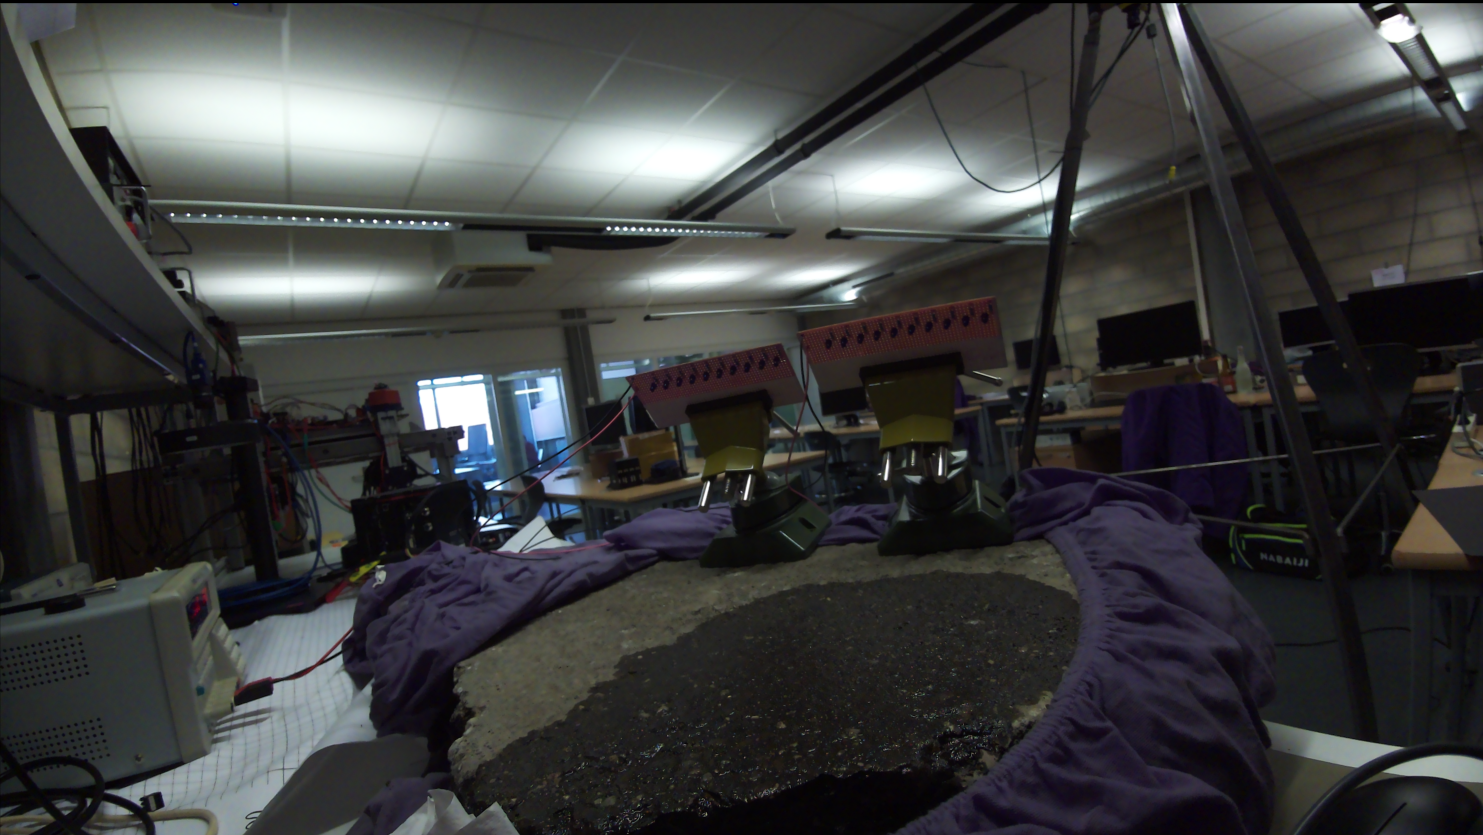
\includegraphics[width=13cm]{assets/figures/camera_vue_couleur1.png}
    \caption{Capture de test - Vue de la scène en couleur}
\end{figure}

Au moment d'effectuer les tests de sensibilités aux IR, tout le matériel n'était pas encore arrivé, notement le filtre de l'objectif ne
laissant passer que les infrarouges. J'ai donc effectué les captures qui vont suivre dans les conditions suivantes:
\begin{itemize}
    \item Lumières éteintes dans la pièce.
    \item Deux lignes de 10 leds IR éclairant en direction de la tâche d'huile de moteur.
    \item Protection contre les lumières parasites du couloir (carton).
    \item Auto-focus sur le centre de l'image
    \item Temps d'exposition: 5000[ns]. (déterminé expérimentalement avec plusieurs captures)
\end{itemize}
Avec ce setup, j'ai effectué plusieurs captures en faisant varier la position de l'éclairage par rapport à la tâche d'huile et la caméra.
J'ai obtenu différents résultats, plus ou moins utilisables.\\
Ci-dessous, un exemple d'éclairage orienté "contre" la caméra selon la figure suivante:\\
\begin{figure}[H]
    \centering
    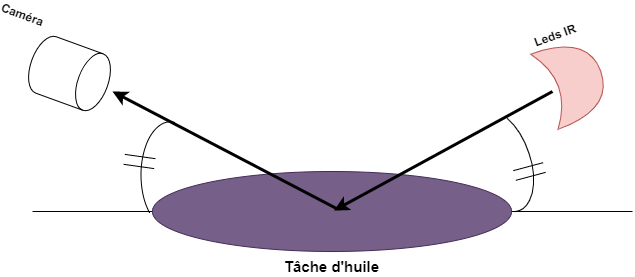
\includegraphics[width=13cm]{assets/figures/eclairage_contre_camera.png}
    \caption{Schéma de capture - Eclairage contre la camera}
\end{figure}


\begin{figure}[H]
    \centering
    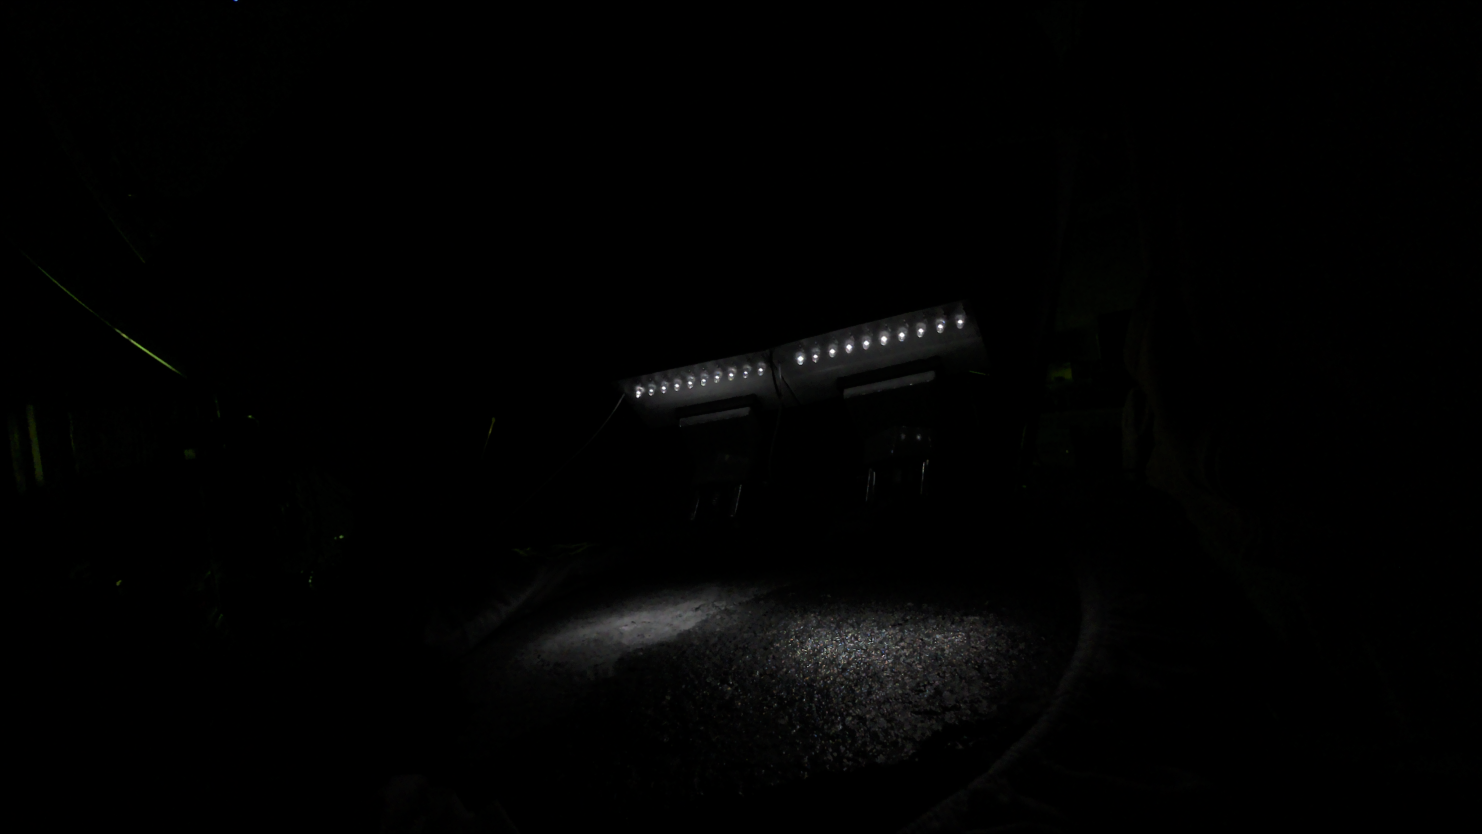
\includegraphics[width=13cm]{assets/figures/eclairage_face1.png}
    \caption{Capture de test - éclairage de face 1}
\end{figure}
\begin{figure}[H]
    \centering
    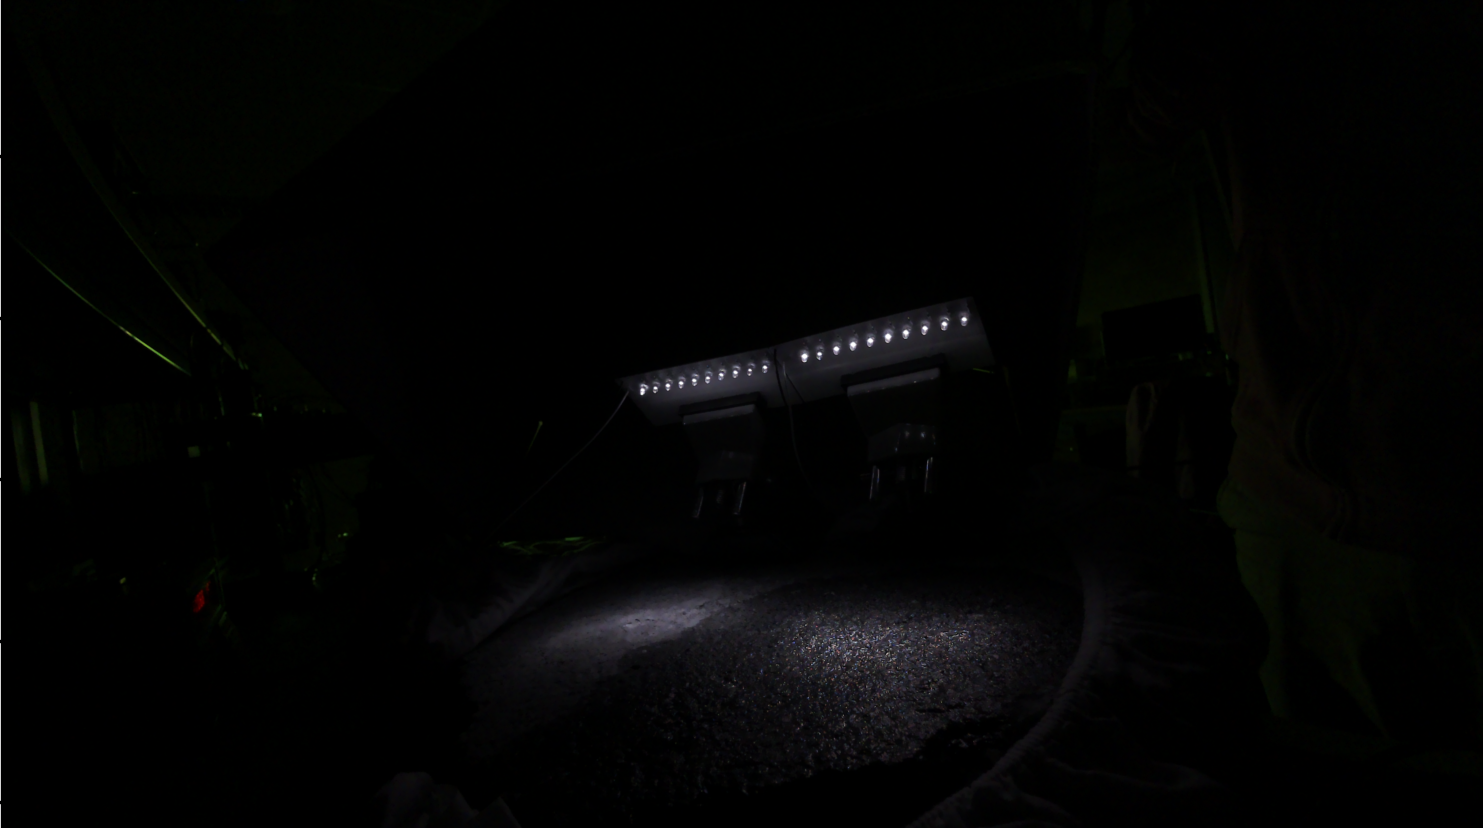
\includegraphics[width=13cm]{assets/figures/eclairage_face2.png}
    \caption{Capture de test - éclairage de face 2}
\end{figure}

On observe que la route et l'huile reflètent les leds IR, à l'oeil nu la différence est notable, mais l'analyse avec un soft peut s'avérer compliquée.\\
Ci-dessous, un exemple d'éclairage orienté perpendiculairement à la route selon la figure suivante:
\begin{figure}[H]
    \centering
    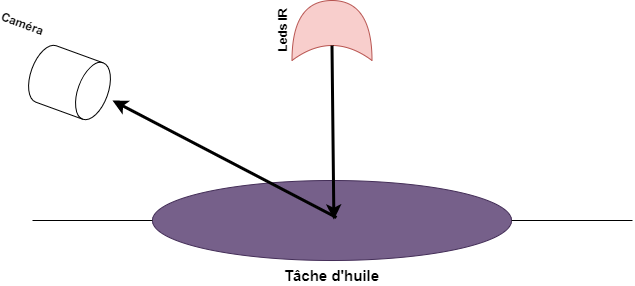
\includegraphics[width=13cm]{assets/figures/eclairage_perpendiculaire.png}
    \caption{Schéma de capture - Eclairage perpendiculaire à la route}
\end{figure}

\begin{figure}[H]
    \centering
    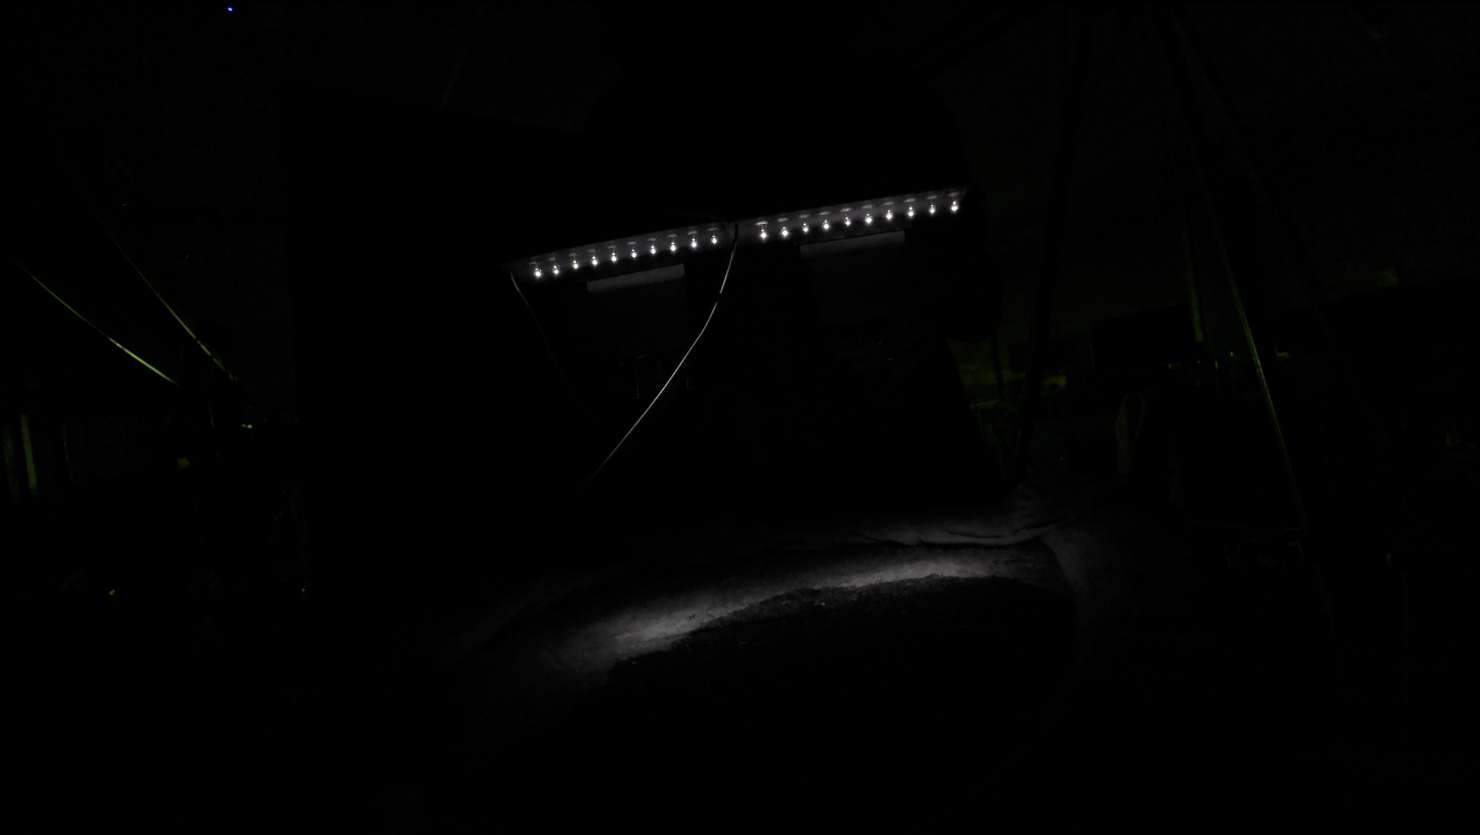
\includegraphics[width=13cm]{assets/figures/eclairage_perpendiculaire1.png}
    \caption{Capture de test - Eclairage perpendiculaire 1}
\end{figure}

\begin{figure}[H]
    \centering
    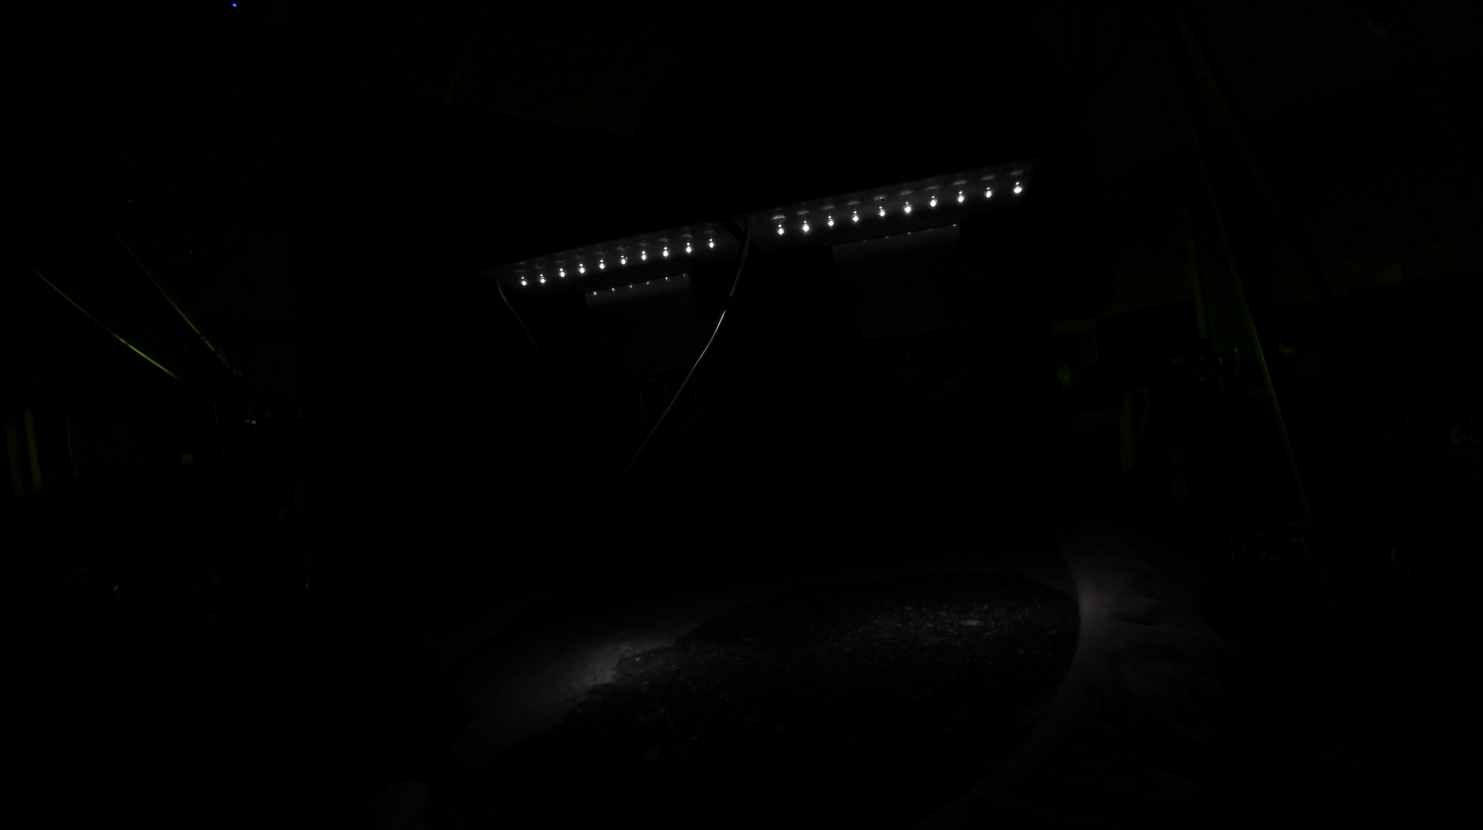
\includegraphics[width=13cm]{assets/figures/eclairage_perpendiculaire2.png}
    \caption{Capture de test - Eclairage perpendiculaire 2}
\end{figure}

\begin{figure}[H]
    \centering
    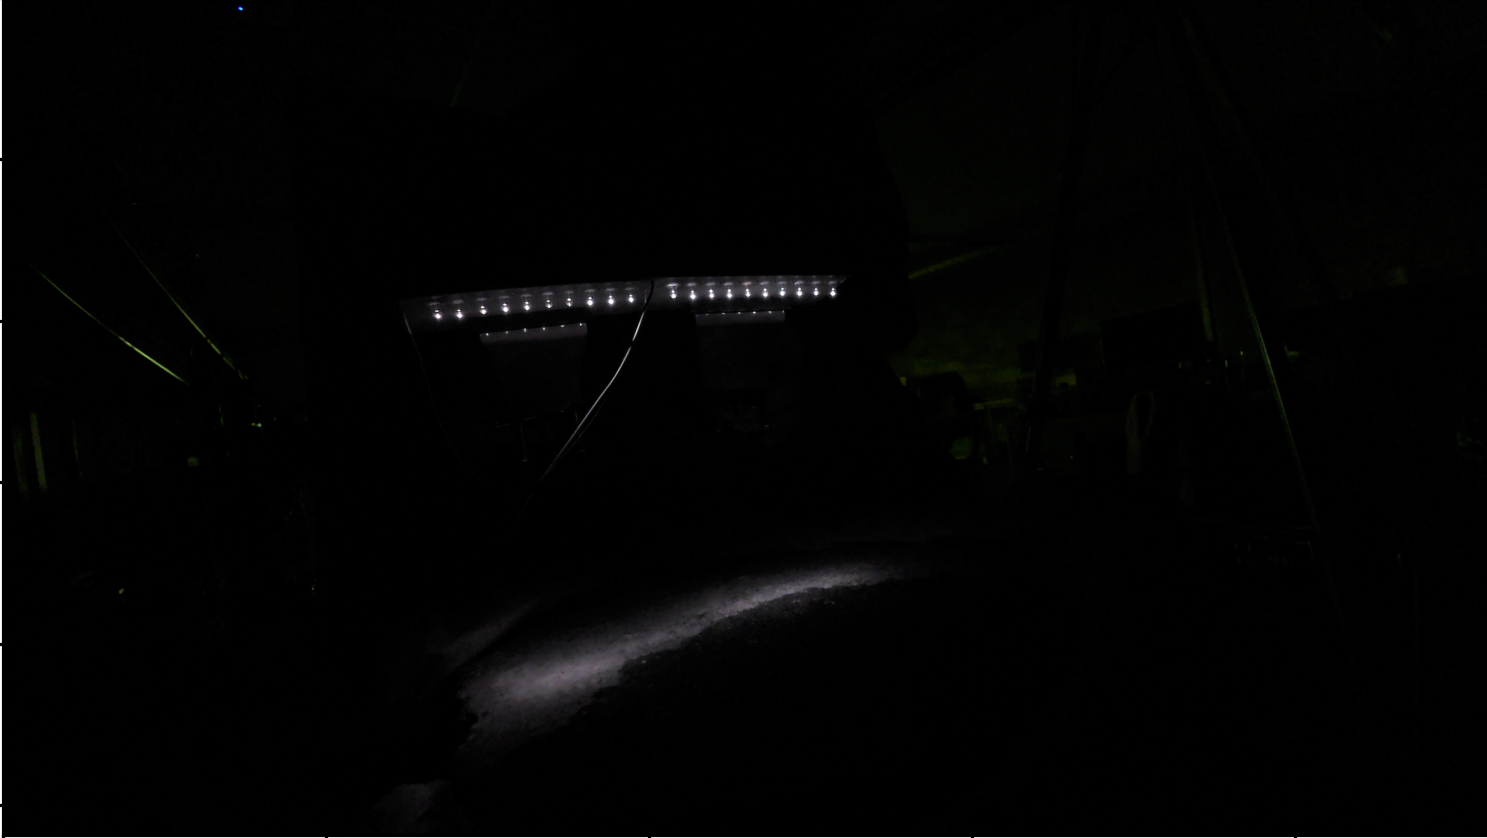
\includegraphics[width=13cm]{assets/figures/eclairage_perpendiculaire3.png}
    \caption{Capture de test - Eclairage perpendiculaire 3}
\end{figure}
On observe que la route diffuse, dans une moindre mesure, l'éclairage des leds IR, là ou l'huile semble absorber les rayonnements. On arrive
assez facilement à différencier le clair de la route et le foncé de l'huile. La mise en place d'un software de détection est envisageable avec un éclairage basé sur ce schéma.

Faire un test avec l'éclairage derrière la caméra

\section{Installation}
\subsection{Eclairage}

\subsection{Caméra}

\section{Programme}
\subsection{Traitement de l'image}
\subsection{Communication}
